\chapter{Introduction}
\label{chap:introduction}
%%%%%%%%%%%%%%%%%%%%%%%%%%%%%%%%%%%%%%%%%%%%%%%%%%%%%%%%%%%%%%%
% OUTLINE FOR INTRODUCTION 
% Segev Outline for Introduction

% SN classification & Identification: Why important?
% Spectra as "gold standard" for classifiers 
% Attempt at spectroscopic classification
% Madgwich et al, Gravr et al (2013), Bovan et al, Mathukrishna et al (2019)
% AI/ ML approach: why better, possibly? 
% What problems does it solve
% what will you be looking at 
% i.e. de-redshifted vs not, subtypeclassification vs none, etc.
% "We will explore the following questions:
%%%%%%%%%%%%%%%%%%%%%%%%%%%%%%%%%%%%%%%%%%%%%%%%%%%%%%%%%%%%%%%

\begin{comment}
-------------------------------------
SYB Comments:
- There is a long history of naked-eye observations of supernovae that predates the invention of the telescope. The most well-known is probably SN 1054, which we now observe as the Crab Nebula.
- Despite millennia of observations, the nature of these explosions was not really understood until the 1930s. It might be interesting to discuss why.
- You don't explain what supernovae are: the end stage of the life-cycle of a massive star (usually $>8 M_\odot$). More rarely (about 1/3 of the time) they are explosions in binary systems involving one WD star + a massive companion sharing a stellar envelope.
- You can work these facts in, with sufficient citations.
\end{comment}

% 
% SB: don't take this the wrong way but the text below is a bit cheesy.
% Maybe a bit of rephrasing is needed (suggestion below).
%
% When observing the night sky, viewers frequently encounter objects that 
% are unexpected. Throughout history, objects appearing out of seemingly nowhere lit 
% up regions of the night sky for a couple of weeks, only to disappear back 
% into the faint glow of the surrounding stars. 
%
Bright astrophysical transients such as novae and supernovae have been observed with naked-eye observations for millennia, but only in the past 130 years, with the advent of astrophysical imaging and spectroscopy and the advance of nuclear physics, have we been able to produce a taxonomy of transients. 
%
For example, in 1885 and 1895, two intensely bright transients were observed for the first time through telescopes, but astronomers were unable to definitively identify their origin \parencite{deVaucouleurs1985, Schaefer1995}. In the 1930s, these objects were eventually named `supernovae' (SNe) by Walter Baade and Fritz Zwicky, who were the first to suggest that these events were the cataclysmic death of stars, and predicted the remaining object to be a cooling neutron star \parencite{Baade1934}. Since then, astronomers 
have defined SNe to be the result of either the core-collapse of stars with a mass $\gtrsim 8M_\odot$, or a thermonuclear explosion in binary star systems involving a white dwarf sharing a stellar envelope with a larger star \parencite{Filippenko1997}. 

\section{Supernova Classification}
\label{sec:supernova-classification}
SNe have traditionally been classified based on their spectra starting with 
\textcite{Minkowski1941}, who first classified SNe into two groups based on the
presence or absence of hydrogen lines. This evolved into 
the current classification scheme, which is based on the presence
or absence of hydrogen and silicon in the spectra of SNe (Figure~\ref{fig:sn-classification}). 

\begin{figure}[t]
    \centering
    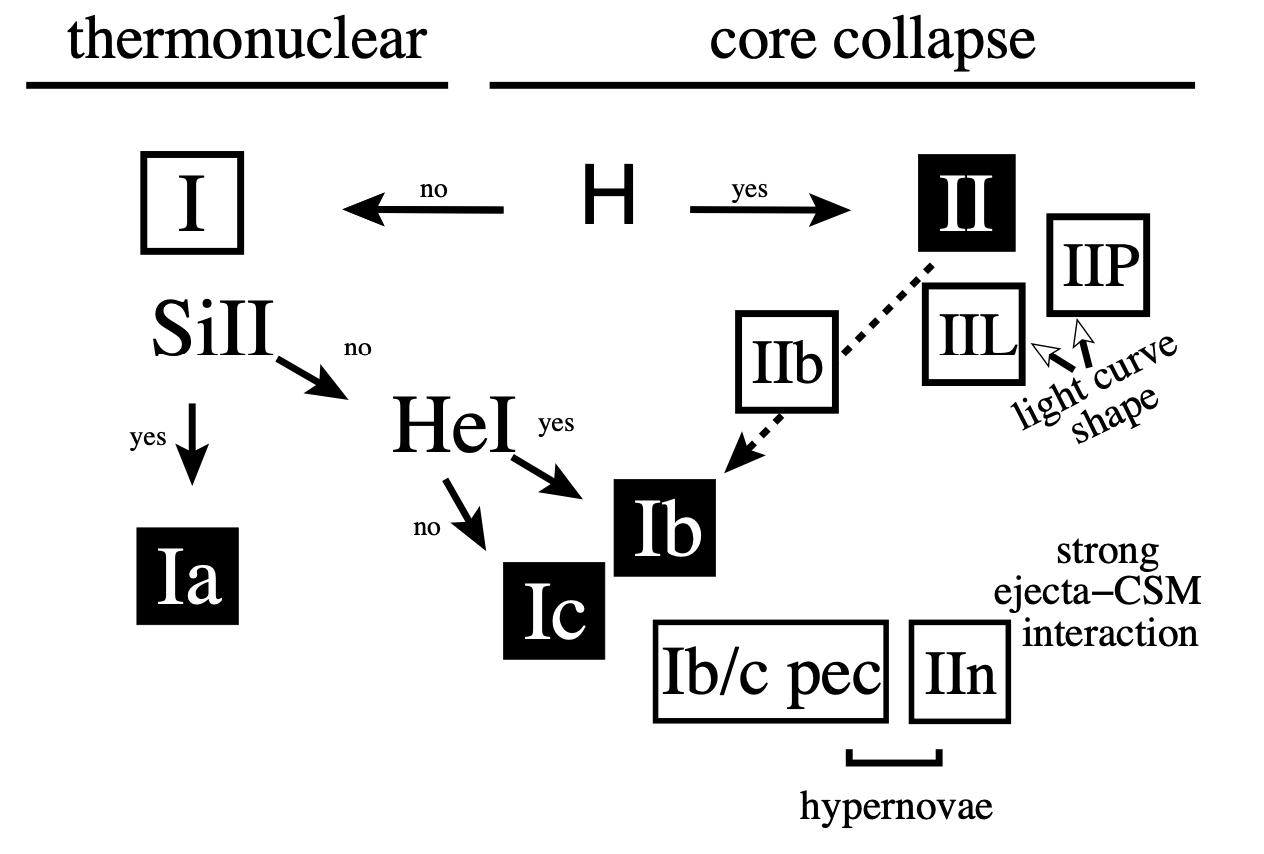
\includegraphics[width=0.8\linewidth]{figures/supernova_class.png }
    \caption[Supernova Classification]{Supernova classification. The 
    classification scheme is based on the presence or absence of hydrogen and 
    silicon features in the spectra of SNe. Figure from \textcite{Turatto2003}.}
    \label{fig:sn-classification}
\end{figure}

SNe with hydrogen in their spectra are classified as Type II SNe, while those
without hydrogen are classified as Type I. Type I SNe are further
subdivided into Type Ia, Ib, and Ic~\parencite{Turatto2003}. The presence of 
SiII is a distinguishing component in the Type Ia classification, with Ib and Ic 
differentiated by HeI. 

Although divided into three 
subtypes, Type I SNe are caused by two different mechanisms. Type Ia SNe are 
caused by the thermonuclear explosion of a white dwarf star, while Type Ib and Ic 
SNe are caused by the core-collapse of a massive star~\parencite{Filippenko1997}.
Thus Type Ib and Ic SNe are actually more related to Type II SNe,
and are collectively referred to as core-collapse SNe. We now know the physical
origin of the spectral differences between the subtypes: stars stripped of their 
hydrogen envelopes appear as Type Ib SNe, while those stripped of both their 
hydrogen and helium envelopes are classified as Type Ic SNe.

% \section{Supernova Identification}
% \label{sec:supernova-identification}
SNe are important for studying the end stages of massive stars, and because some subtypes have standardizable magnitudes (specifically SNe Ia and II-P) they are used in the cosmological distance ladder. Therefore, merely detecting a supernova is not enough, as astronomers must identify its
type to study the progenitor and, if possible, compute its distance modulus. Generally, a supernova is observed by several 
means, with discovery in photometric observations and classification using follow-up 
spectroscopy (e.g. \textcite{Perlmutter1999} and references therein). This process is time-consuming, requiring not only 
the initial discovery of the supernova but also follow-up observations to determine
the type before it fades away. Due to the large volume of new discoveries and 
the relatively small number of single and multi-object spectrographs suitable for follow-up, only 
about 10\% of discovered SNe receive spectroscopic classification \parencite{TNS}. 

\section{Dark Energy Spectroscopic Instrument}
\label{sec:DESI}
The Dark Energy Spectroscopic Instrument (DESI) is a spectroscopic system located at Kitt Peak National Observatory
in Arizona. Installed at the Mayall 4-m telescope, DESI is fitted with 5,000 fiber positioners and ten 3-arm 
spectrographs capable of resolving the [O II] $\lambda \lambda3726,3729$ doublet used for redshift fits of galaxies \parencite{Guy2023}. 
%
% SB: This is good but flesh out a bit about the survey.
%
% This instrument is currently being used in the DESI Bright Galaxy Survey (BGS) to produce a map of a dark-energy dominated universe with median redshifts of $z \approx 0.2$ \parencite{hahn2022, desicollaboration2016}.
%
\begin{figure}[t]
    \centering
    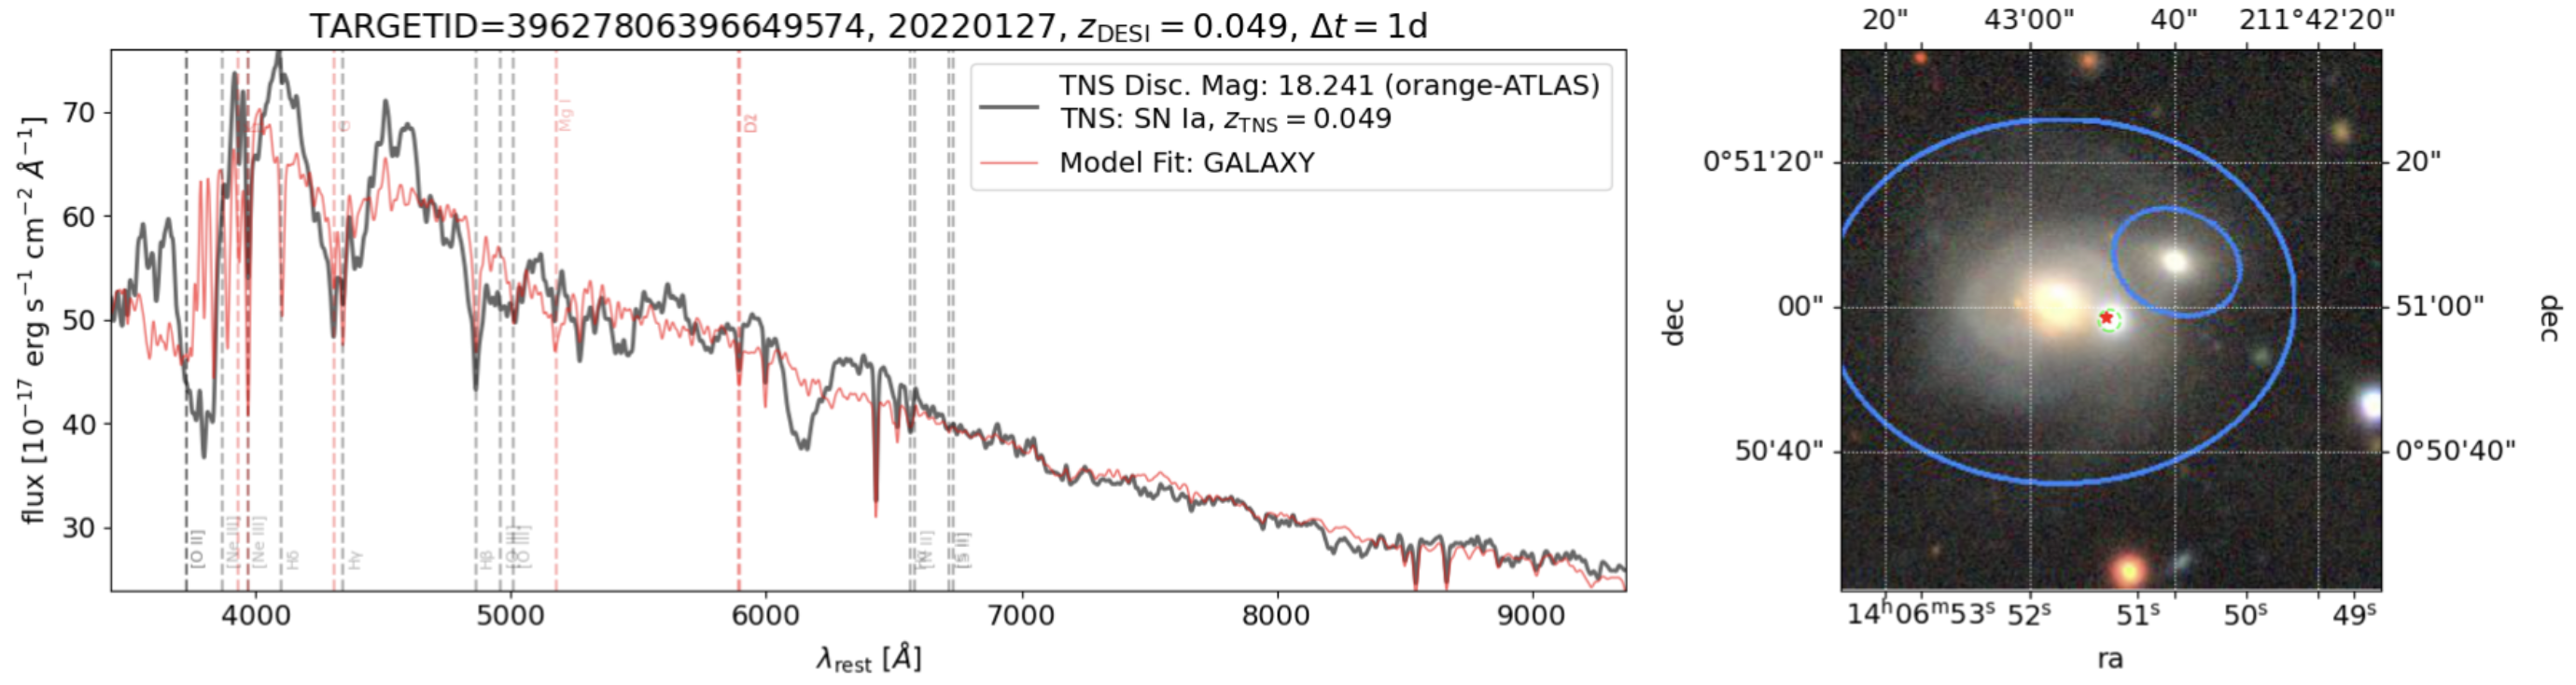
\includegraphics[width=\textwidth]{figures/desi_figures/SNe_Detection.png}
    \caption[Publicly Classified SNe captured by DESI]{DESI host galaxy spectrum contaminated by a Type Ia supernova (January 2022). The right panel shows the image of the host galaxy, with the red star indicating the position of the DESI fiber. Independent spectroscopic follow-up reported to the TNS public database confirmed this is an SN Ia.}
    \label{fig:desi_supernova}
\end{figure}

The DESI survey focuses on four classes of targets: 14 million bright galaxies\footnote{The BGS contains galaxies with $r$-band magnitudes above 19.5.} in a Bright Galaxy Survey (BGS) at redshifts $z<0.5$; 8 million luminous red galaxies (LRGs) at redshifts $0.4<z<1.2$; 17 million emission line galaxies (ELGs) at $0.6<z<1.6$; and 3 million quasi-stellar objects (QSOs) between $0.9<z<4$. In this work, we will focus on the Bright Galaxy Survey, which is observing host galaxies with a median redshift of $z\approx0.2$ \parencite{desicollaboration2016, hahn2022}.

DESI began its main survey in May 2021. Over the five-year span of observations, DESI will inevitably observe host galaxies with active SNe, leading to 
contaminated spectra. The BGS may contain as many as $\sim10^5$ serendipitously observed supernova 
\parencite{desicollaboration2016}. An example of a supernova observed in a BGS host by DESI and with an independent spectroscopic classification is shown in 
Figure~\ref{fig:desi_supernova}.
\begin{figure}[t!]
    \centering
    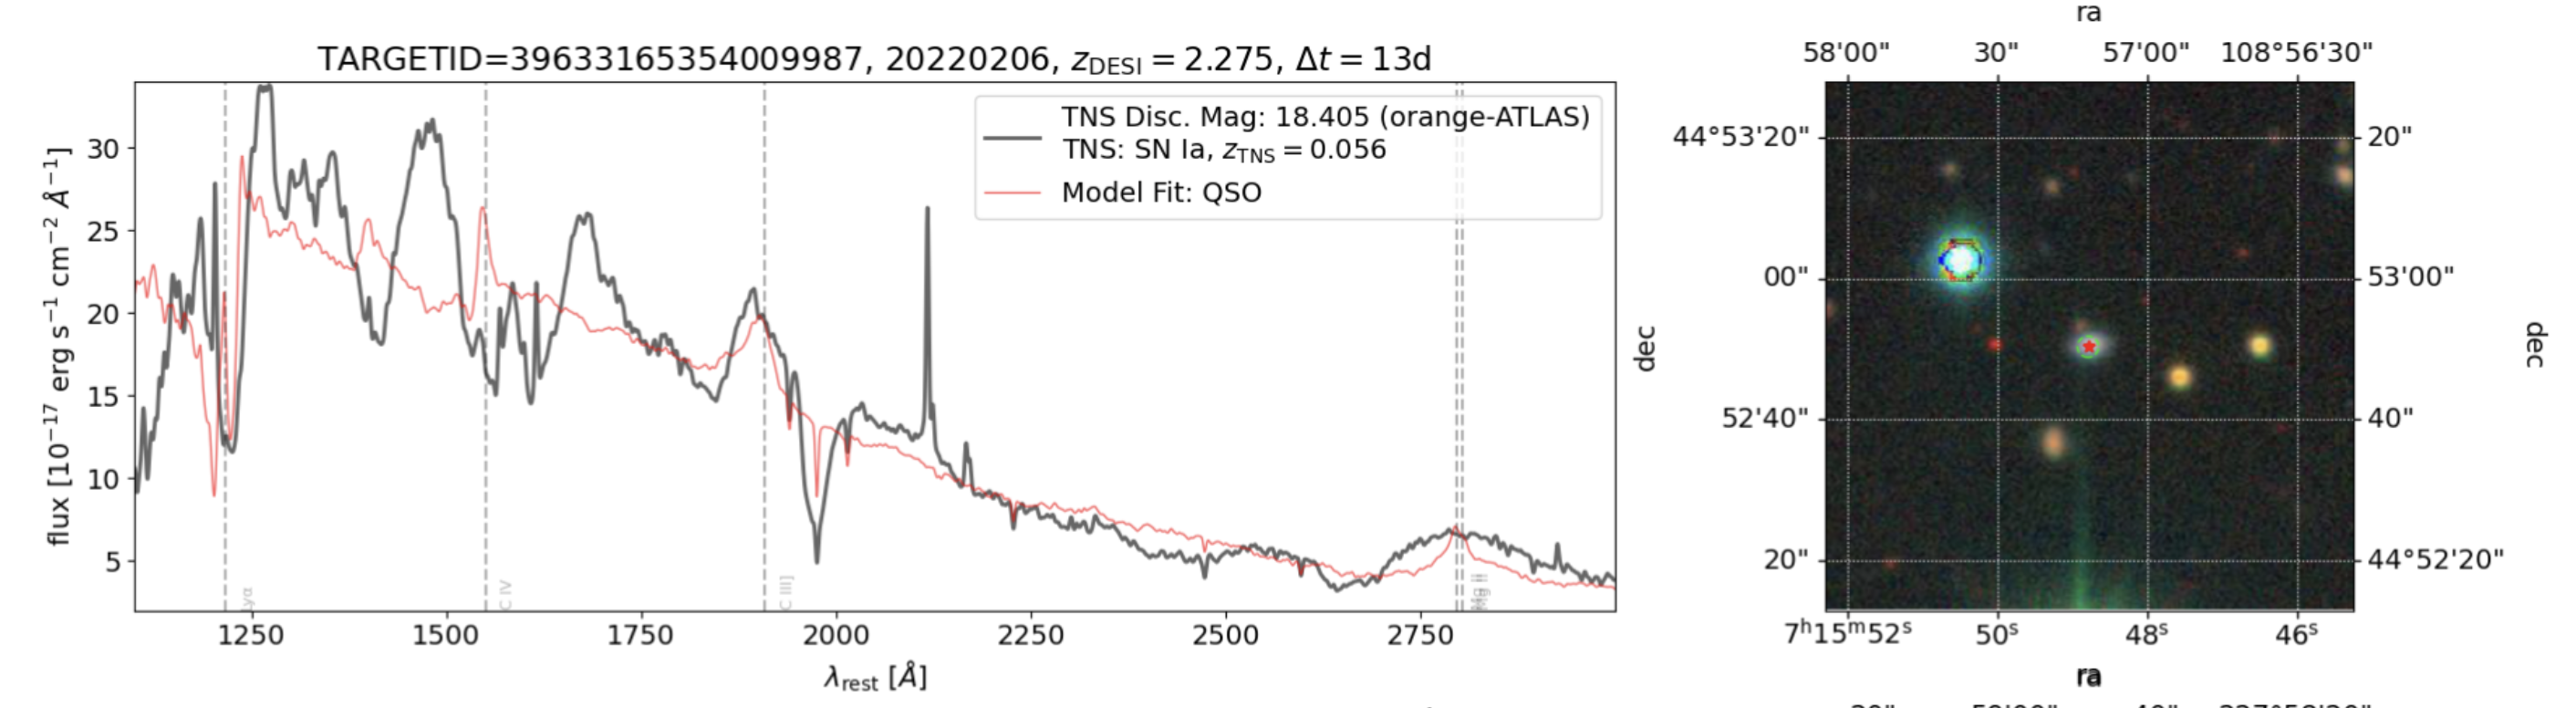
\includegraphics[width=\textwidth]{figures/desi_figures/SNe_detection_desifail.png}
    \caption[SNe Influencing DESI Redshift Fit]{DESI host galaxy spectrum contaminated by a Type Ia supernova (February 2022). The right panel shows the image of the host galaxy, with the red star indicating the position of the DESI fiber. Independent spectroscopic follow-up reported to the TNS public database confirmed this is an SN Ia. Note the extremely poor redshift fit provided by the DESI pipeline.}
    \label{fig:desi_supernova_fail}
\end{figure}

%
% SB: the following sentence is OK but I'd add that the real interest is just getting spectroscopic classification "for free" when we're already observing millions of bright galaxies.
%
% Transients of any kind run the risk of influencing the redshift fit provided by DESI, making transient detection and identification of upmost importance to the quality of the pipeline. The difficulties in ensuring follow-up observations of possible SNe candidates prompts the development of autonomous techniques geared towards the discovery and classification of these targets serendipitously. 
%
The presence of transients in DESI spectra is a contaminant for the survey's dark energy program, since the transient can cause a catastrophic failure in the redshift fit, as shown in Figure~\ref{fig:desi_supernova_fail}. Thus it is useful to identify these contaminants whenever possible. Moreover, the serendipitous observation of supernovae is inherently useful since the spectroscopy provides an opportunity to classify {\sl most} types of supernovae without requiring additional follow-up. Both of these factors motivate this study.


\section{Past Approaches to Spectroscopic Identification}
\label{sec:PrevApproach}


% SB: here you should refer to past publications.
% See https://docs.google.com/presentation/d/1zqoEVMrWbBP5k41gdjUEKioLE4J0vhu0vAzKEg4pROM/edit?usp=sharing
%
The idea to search for active transients in spectroscopic data sets is not new; see, for example, \textcite{Madgwick2003}, \textcite{Graur2013}, \textcite{Baron2017}, \textcite{Muthukrishna2019}, and \textcite{Davison2022}.
%
Until the past 5 years, most spectroscopic supernova identification algorithms would compare observations against supernova spectral templates; more recent searches have applied machine learning techniques. In nearly all cases, the searches proceed by characterizing and subtracting the galactic continuum of the host galaxies and then fitting the template to the residual spectra or running a machine-learning algorithm on the residual spectra.

The use of templates and residual spectra, while robust and easy to understand, leads to several computational inefficiencies. First, the host galaxy continuum must be fit accurately in the presence of a possibly dominant transient. An incorrect fit, 
regardless of the presence of a supernova, can lead to misclassification. Second, even if 
it is assumed that the residual spectrum contains only a supernova, a template search must include all of the subtypes of 
SNe adjusted for all possible redshifts appropriate for the targets. In addition, the classification of 
SNe is also time-dependent, so the evolution of each subtype must also be included in each template. An 
example SN Ia model showing the spectral evolution is provided in Figure~\ref{fig:sne_template}.

\begin{figure}[t]
    \centering
    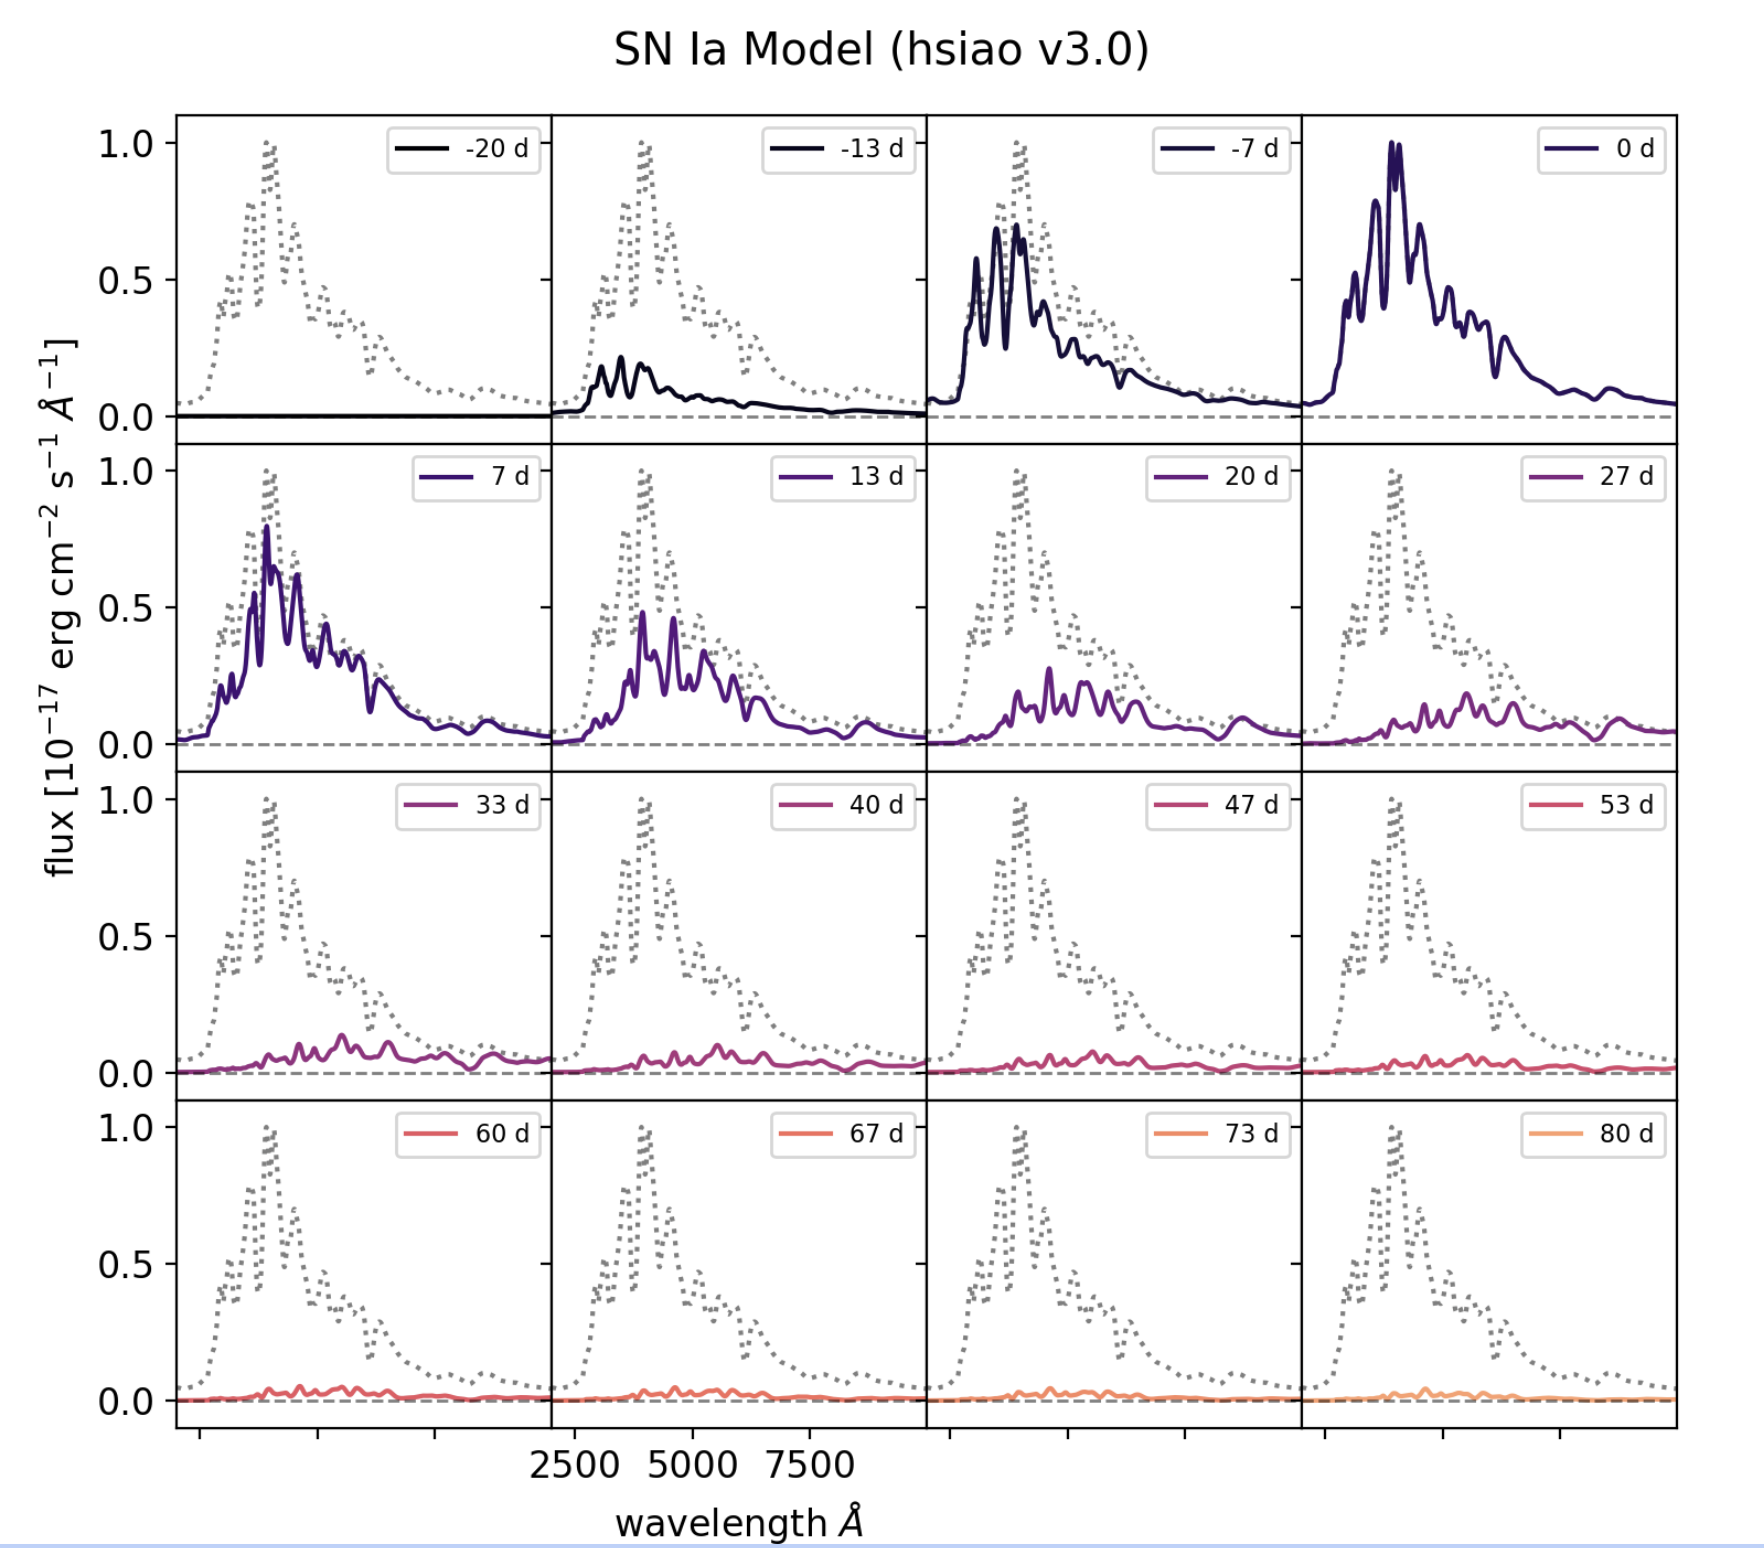
\includegraphics[width=.8\textwidth]{figures/desi_figures/snia_templates.png}
    \caption[Spectral Template of SN Ia SNe]{Spectral model of a SN Ia shown over the course of its evolution, from 20 days before peak brightness to 80 days after. Adapted from \textcite{DESIpresentation}.}
    \label{fig:sne_template}
\end{figure}

% https://docs.google.com/presentation/d/14i0USbCQ93Mkn1T9aUK5pG24bi5bRfBhM3aVsL1Ya0U/edit?usp=sharing
% -- Look at spectra examples
% -- Look at motivation for no-redshift corrected transient classification

% https://docs.google.com/presentation/d/1zqoEVMrWbBP5k41gdjUEKioLE4J0vhu0vAzKEg4pROM/edit?usp=sharing
% -- An old presentation from 2020 that lists some past approaches to spectroscopic classification.
% -- Supernova tempates and compared them 
%   - Fit forgrown spectra from galaxy, fit residual spectrum. CHi^2 fit looks good?you discover it
% -- type IA evolution
%   - You can't just compare to one, you need to compare to A BUNCH because of time 
%   - So you want to compare to every template?? Convolve at different redshifts??
%   - SUUUPER expensive. ML/AI is just... better. 


\begin{comment}
% SB Comments:
% You want to motivate this in a couple of ways.
% 1) Because spectroscopic follow-up is tough, it's worthwhile to try to discover SNe serendipitously in spectra rather than only wait for discoveries in imaging surveys.
% 2) The issue with spectroscopic discovery is that you have potentially thousands of templates to compare against (all the different subtypes * all the variants of the subtypes * the spectral evolution of each variant * convolution vs redshift). Very computationally expensive!

% I suggest you give some background on previous approaches before jumping right into AI/ML.
% See the early slides in \href{https://docs.google.com/presentation/d/1zqoEVMrWbBP5k41gdjUEKioLE4J0vhu0vAzKEg4pROM/edit?usp=sharing}{this Google slideshow}.
\end{comment}

\section{Supernova Classification with Machine Learning}
\label{sec:supernova-classification-with-machine-learning}
Machine learning (ML) has been applied broadly to different fields for its flexibility 
and ability to find patterns in data. The emergence of Deep Learning (DL) has
allowed ML to be applied to tasks such as image
classification~\parencite{krizhevsky2012}, speech recognition~\parencite{Nassif2019},
and natural language processing~\parencite{Mikolov2013}. ML and DL 
have recently been applied to astronomy, with promising results. \textcite{Gauci2010} used 
a random forest algorithm  to distinguish between spiral, elliptical, and irregular galaxies, 
and \textcite{Becker2021} used a convolutional neural network (CNN) to classify the morphology of
radio galaxies. CNNs found success in working within the DESI collaboration, with 
\textcite{parks2018} using the architecture to detect strong emission lines.  
These techniques have also been applied to the classification of SNe. 
\textcite{Mller2016} used a CNN to classify SNe into Type Ia and non-Ia SNe, and \textcite{Muthukrishna2019} and \textcite{Davison2022} further extended the classification to identify core-collapse subtypes.

\begin{comment}
\section{Problem Statement}
This work will explore the following questions: how can we adapt novel deep learning 
techniques to classify SNe in the DESI dataset? Can we use this architecture to 
classify SNe into their respective subtypes accurately? And how can we decrease the amount of 
pre-processing required to classify these SNe accurately? In the following chapters,
we describe the Deep Learning techniques adopted to answer this problem (Ch. 2);
the training procedure for building our classification network (Ch. 3);
and the results using simulated DESI spectra that were resampled from actual 
DESI measurements performed in 2021 and 2022 (Ch. 4).
\end{comment}

Previous attempts at using ML algorithms for transient detection specifically on DESI 
spectra have been conducted by \textcite{rubenzahl2018, wasserman2021, Sepeku2022}. The classifiers 
presented by \textcite{wasserman2021, Sepeku2022} were 
shown to be capable of high precision (further explained in Section~\ref{sec:CNNspectra}), 
but only after pipeline-dependent preprocessing and extensive cutting based on model certainty.
An alternative model based on the vision transformer (ViT) architecture is proposed here to 
solve these shortcomings. Aptly named the ``Spectral ViT,'' this model seeks to 
classify SNe into their respective subtypes with comparable precision and higher 
recall compared to previous classifiers, without dependence on the DESI redshift fit for pre-processing. 

In Chapter~\ref{chap:DLTechniques}, the deep learning techniques used throughout the study 
are explained in detail, while Chapter~\ref{chap:methods} describes the creation and training 
of the Spectral ViT. The results of the study are discussed in Chapter~\ref{chap:results}, with 
future research and applications of this model presented in Chapter~\ref{chap:conclusions}. 



